\section{General Definitions}
\label{sec:general_definitions}

This chapter provides a formal definition of the Traveling Salesman Problem (TSP) and gives an overview of existing approaches to solve it. Moreover, it introduces genetic algorithms with their main phases and discusses how they can be used to solve the TSP.\par 

\subsection{The Traveling Salesman Problem}
\label{subsec:tsp}

The Traveling Salesman Problem (TSP) is the problem where a salesperson needs to visit customers which are located in different cities and looks for a shortest round trip to fulfill this issue as defined by \citeauthor{hoos2004stochastic} (see \cite{hoos2004stochastic}). \par 

The TSP is typically modeled using a directed, edge-weighted graph $K_{n} = (V, E)$ (see \cite{hoos2004stochastic}, \cite{knust2020script}), where each node $v \in V$ represents one of $n$ cities (i.e., $|V| = n$). An edge $e = (u, v) \in E$ between two nodes $u, v \in V$  represents a connection between the corresponding cities, and the weight on this edge represents the distance between them. These edge weights are represented by the cost function $c : E \rightarrow \mathbb{Z}$. \par 
In our implementation, the cost function is represented by a distance matrix $D$, where entries $d_{ij}$ represent the distance $d(i, j)$ between cities $i$ and $j$. That is, the cost function $c$ is defined as $c(i, j) := d_{ij}$. If $D$ is \textit{symmetric}, that is, for all $ i, j \in V: d_{ij} = d_{ji}$, the corresponding TSP instance is called \textit{symmetric} as well.  If $D$ is not symmetric, than the corresponding TSP instance is called \textit{asymmetric}. $D$ is said to satisfy the triangle inequality if and only if for all $i, j, k \in V: d_{ij} + d_{jk} \geq d_{ik}$. This occurs in case of Euclidean TSP instances with $V$ as a set of points in $\mathbb{R}^{2}$  and $d_{ij}$ as the length of the straight line segment between $i$ and $j$ as defined by \citeauthor{laporte1992traveling} (see \cite{laporte1992traveling}). Note that in our experiments, we only consider symmetric Euclidean TSP instances.

We call two nodes \textit{adjacent} if they are connected by an edge. Two edges are called \textit{incident} if they share a node. Also, a node and an edge are called \textit{incident} if the edge starts or ends at this node. \par 

A round tour through all cities is represented by a cyclic permutation $\pi = (\pi_{1}, ..., \pi_{n})$ of vertices, where $\pi_{n+1} := \pi_{1}$ (see \cite{knust2020script}). Such a cyclic permutation is also known as a \textit{Hamiltonian cycle}. An optimal solution for the TSP consists of a cyclic permutation $\pi$ which minimizes the overall costs $c(\pi) := \sum_{i=1}^{n} c(\pi_{i}, \pi_{i + 1})$. An example of a symmetric TSP instance in the form of a graph is given in Figure \ref{2_1_graph_example}. One can use different start cities and visit the cities in two directions as the given instance is symmetric. This results in eight tours which correspond to the same optimal solution. \mbox{Without} loss of generality, we take the city 0 as a start city. As the instance is symmetric, we can go into two directions getting optimal tours $\pi_{1} = (0,2,3,1)$ and $\pi_{2} = (0,1,3,2)$. \\


\begin{figure}[htp] \centering
	\centering
	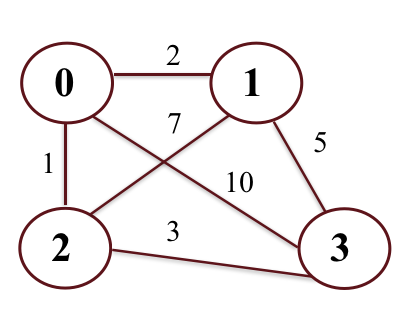
\includegraphics[width=0.4\textwidth]{2_1_graph_example}
	\caption{An example of a symmetric TSP instance with four cities.}
	\label{2_1_graph_example}
\end{figure}

 Generally speaking, there are two main ways to solve the TSP, namely exact and approximate algorithms. Exact algorithms basically consider all possible solutions in order to choose an optimal one, resulting in enormous computational costs. The most direct approach would be to try all possible cyclic permutations. For a fully connected graph with $n$ nodes, their number is $(n - 1)!$, resulting in the runtime ${O}(n!)$, the factorial of the number of cities. This growth in runtime, caused by increasing the number of cities $n$, is even faster than the exponential growth, as ${O}(n!)\supset {O}(2^{n})$. This makes the problem of finding optimal round tour quite challenging. Of course, there are some approaches which improve the runtime, as, for instance, the dynamic programming approach proposed by \citeauthor{bellman1962dynamic} \cite{bellman1962dynamic} with the runtime ${O}(n^{2}2^{n})$. However, the growth in runtime still remains exponential. Therefore, running an exact algorithm for hours on a powerful computer may not be very cost-effective. In terms of quality and speed, solving the problem with approximate algorithms (also called heuristics) can be more feasible. \par 
 
 Approximate algorithms can be classified into three main types, namely:\par
 \begin{itemize}
 	\item Construction heuristics
 	\item Improvement heuristics
 	\item Composite heuristics	 
 \end{itemize}

  \textbf{Construction} procedures start from an initial partial tour (usually a randomly chosen city) and iteratively extend it until a complete round tour has been constructed. A more detailed description of them is given in Chapter \ref{sec:heuristics}.\par
  
  \textbf{Improvement} procedures start from a complete tour and try to reduce its length while ensuring that the result is still a valid tour. \citeauthor{gendreau2005metaheuristics} \cite{gendreau2005metaheuristics} have divided them further into \textit{single-solution heuristics} and \textit{population heuristics}. While the first group works with a single solution at a time, population heuristics work with multiple solutions evolving during the search process. One of the representatives of the latter group, namely genetic algorithms, will be discussed in the following section.\par 

  At last, \textbf{composite} approaches can be seen as a combination of construction and improvement procedures: They begin with a tour construction procedure to build an initial tour which is then refined using tour improvement procedures. 
  
  The classification of the above mentioned approaches is given in Figure \ref{2_1_approaches_to_tsp_detailed} provided with some examples for each type.
 
 \begin{figure}[htp] \centering
 	\centering
 	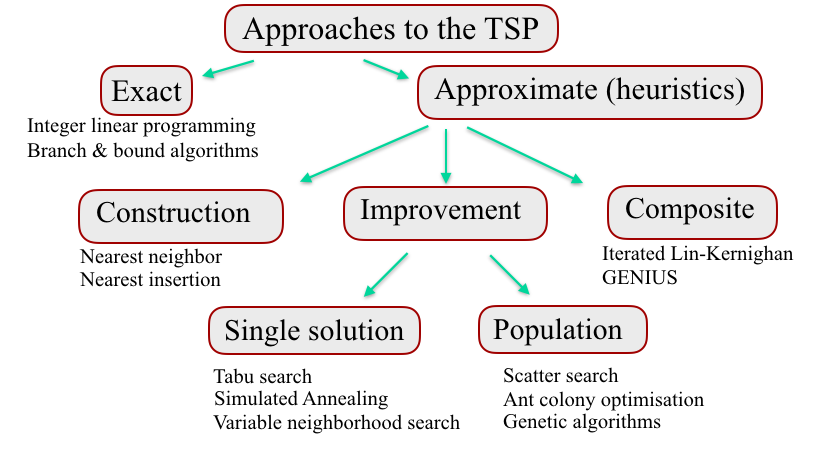
\includegraphics[width=0.7\textwidth]{2_1_approaches_to_tsp_detailed}
 	\caption{Existing approaches to solve the TSP (based on classifications given by \citeauthor{potvin1996genetic} \cite{potvin1996genetic}, \citeauthor{gendreau2005metaheuristics} \cite{gendreau2005metaheuristics}).}
 	\label{2_1_approaches_to_tsp_detailed}
 \end{figure}
 
\subsection{Genetic Algorithms}
\label{subsec:ga}

Being a widely known metaheuristic, genetic algorithms are an approach for a randomized search introduced by \citeauthor{holland1975adaptation} \cite{holland1975adaptation} which is based on the Darwinian principle of natural selection.  Feasible solutions (usually encapsulated in the form of "chromosomes") build a population of a chosen finite size. A so-called fitness function assigns to each chromosome a fitness value which represents the quality of the corresponding solution. The fittest chromosomes of the population are more likely to be chosen by selection operators to produce offspring for the next generation. These new offspring chromosomes are created by applying crossover operators (which combine genetic material from two parents) and mutation operators (which produce small random perturbations with a given probability).  Starting from a randomly or heuristically generated initial population, this process repeats until the defined stop criteria are reached. This general formulation of genetic algorithms is inspired by the description provided by \citeauthor{potvin1996genetic} \cite{potvin1996genetic} and \citeauthor{gendreau2005metaheuristics} \cite{gendreau2005metaheuristics}. It is illustrated in Figure \ref{ga_procedure}.

 \begin{figure}[htp] \centering
	\centering
	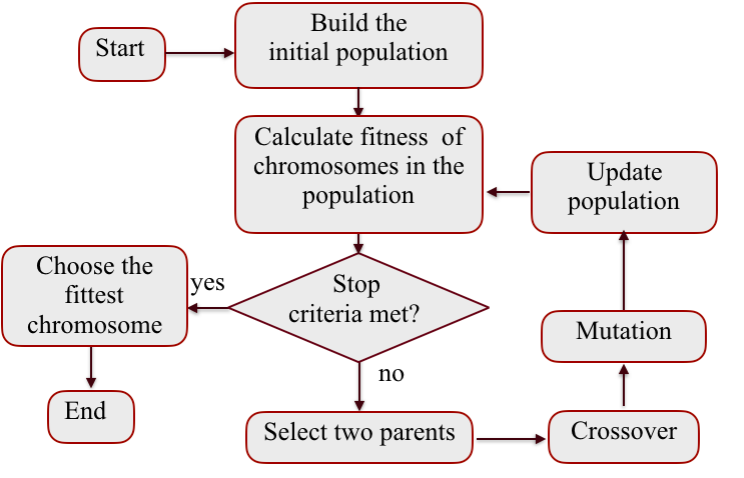
\includegraphics[width=0.7\textwidth]{ga_procedure}
	\caption{The general procedure of an genetic algorithm.}
	\label{ga_procedure}
\end{figure}

This is a genetic algorithm template, where each phase is defined in a rather abstract way. In a specific domain, there is a number of open questions which have to be answered. First of all, which type of representation should be used? Each domain can have its unique types which have to be considered. How should the population be initialized? There are two main options to do that, namely creating chromosomes randomly or initializing them by applying heuristics. Another question to be answered is whether the size of the population remains fixed or whether the population can grow dynamically. In the first case, it is necessary to define this fixed size and in the latter case, one needs to specify to which extent the population can grow. \par 

Another important decision concerns the choice of stop criteria for the algorithm. According to \citeauthor{safe2004stopping} \cite{safe2004stopping}, there are three termination conditions which are typically used: 

 \begin{itemize}
	\item maximum number of iterations (generations),
	\item maximum number of evaluations of the fitness function, and
	\item a low chance of getting significant changes in the next generations.
\end{itemize}

In our experiments, we are going to stop the algorithm after a fixed amount of time. When comparing the results of different setups, we can thus estimate the quality of achieved results per unit of time which can be relevant for practical applications. \par

Further degrees of freedom involve the choice of selection, crossover and mutation operators. Different variants of these operators in the context of the TSP will be introduced in Chapters \ref{sec:selection}, \ref{sec:crossover}, and \ref{sec:mutation}, respectively. Please note that mutation operators are typically used with a certain probability. This probability is another parameter that needs to be determined.\par

Moreover, a decision needs to be made about the way of updating the population: Newly generated offspring chromosomes can replace their parents or not. In the former case, one also needs to specify under which conditions the replacements occur. One more question is whether mutations can be applied to only the offsprings which are produced through crossover, or to any chromosome from the population.\par

The answers to all these questions tend to be domain specific; therefore, they can be addressed using the best practices in the corresponding field. However, this domain knowledge is typically not sufficient for determining all choices. Thus, the unanswered questions can be considered as general parameters for the algorithm which then have to be optimized in order to find the best configuration.\\

From now on, we are going to focus on genetic algorithms for solving the TSP. For this purpose, some specifications have to be made. A feasible solution to a TSP problem is a cyclic permutation of the cities, or in other words, a feasible round tour, where each city appears exactly once. There are different ways to represent such a tour which will be discussed in Chapter \ref{sec:representation_types}. These round tours will be encoded in form of chromosomes which together make up the population. Distances between cities (which in our implementation are given in the form of a distance matrix) serve as a basis for the fitness function. The calculation of the fitness value of a chromosome is based on the length of the round tour it encodes. Please note that as we look for a round tour with minimal length, we need to minimize the whole distance of the tour. In our implementation, the fitness value of a tour corresponds to the length of this tour multiplied by minus one so that we can maximize the fitness function. In this case, the chromosome with the largest fitness value is considered to be the fittest and, correspondingly, the best one. \par